 %!TEX root = main.tex
\chapter{The relevant scales: sizes, energies, concentrations}

\section{Units and dimensions}
Objects and events in the world around us have quantifiable properties such was length, mass, duration, charge, etc.
These nature of these properties are often called dimensions and for each of these dimensions, we have one or several units in which we measure them: grams, meters, seconds etc.
Fundamentally, all these measurements are comparisons between quantities of the same dimension.
We measure the length of an object by comparing it to a stick of a particular length -- one meter.
These units have been agreed upon and are usually chosen to be convenient for a particular use case.
A meter, for example, is roughly one step.
Importantly, we can only compare things of the same dimension: length with length, mass with mass, etc.
There no sense in which you can meaningfully compare a quantities of different dimensions, for example one measured in meters to another one measured in kilograms.

Physical laws, on the other hand, relate quantities of different dimensions to each other.
Take Newton's law:
\begin{equation}
	F = m\times a \quad\quad \mathrm{Force [N]} = \mathrm{mass [kg]}\times \mathrm{acceleration [m/s^2]}
\end{equation}
The unit of force (Newton) is a product of the units of mass (kilogram) and acceleration, which itself as dimension length/time$^2$ and is measured in meter/second$^2$.

Whenever you specify a physical quantity, you have specify the unit!

\section{The relevant scales}
To quantitatively understand how different biological processes and phenomena relate to each other, it is essential to get a sense of the relevant length, force, energy, and concentration scales.
A very useful collection of important quantities is available at \href{http://book.bionumbers.org}{bionumbers.org} by Ron Milo and colleagues.
Once we have identified the relevant scales and sizes, simple reasoning and comparing different scales can already give us quite robust insight into many cell biological properties.

\subsection{How small are things?}
The following table has (very) rough numbers for the different sizes involved

\begin{itemize}
  \item $3\times 10^{-10}$m (0.3nm): height of one DNA base pair
  \item $2\times 10^{-9}$m (2nm): diameter of DNA, typical protein diameter
  \item $2\times 10^{-8}$m (20nm): bacteria phage
  \item $10^{-7}$m (0.1$\mu$m): animal virus
  \item $10^{-6}$m (1$\mu$m): bacterial cell
  \item $2\times 10^{-6}$m (2$\mu$m): yeast cell nuclei
  \item $10^{-5}$m (10$\mu$m): eukaryotic cell
\end{itemize}

\begin{figure}[h]
	\centering
	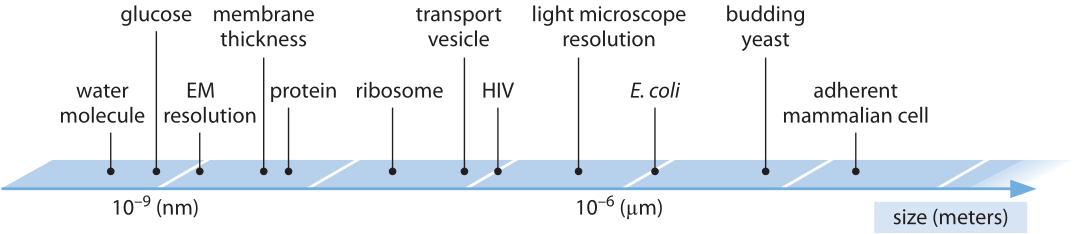
\includegraphics[width=\textwidth]{100-f1-LengthScalesGraphic-14.png}
	\caption{The range of linear dimensions relevant in a cell from \href{http://book.bionumbers.org/size-and-geometry-introduction/}{book.bionumbers.org}}
	\label{fig:length_scales}
\end{figure}

With this huge range of linear dimensions, volume and mass vary over a much larger range still.
It is useful to remember: One liter is $10^{-3}m^3$, one milliliter is a $cm^3$ (the size of an eppendorf tube), one femto liter is $\mu m^3$. One gram of water is roughly one milliliter.
Using the length scales above, we get the following rough volume scales for biological entities (there is obviously a lot of variation between cell and virus types).

\begin{itemize}
  \item $10^{-20}$l: volume of a bacteria phage
  \item $10^{-15}$l (1fl): volume of a bacterial cell
  \item $10^{-12}$g (1pg): weight of a bacterial cell
  \item $10^{-12}$l (1pl): volume of a eukaryotic cell
\end{itemize}

Humans weigh roughly 100kg (100l volume) and most of ``human stuff'' is made from cells. Given the rough weight of a cell, we estimate $10^{14}$ human cells in the human body.
The true number is closer to $10^{13}$, but this discrepancy is within the accuracy of our calculation.
Furthermore, we immediately see that a comparable number of bacterial cells will contribute rather little to the total weight since the individual cell is 1000-fold lighter.


\subsection{Typical genome sizes}
Genome sizes vary enormously among species.

\begin{itemize}
  \item $3\times 10^{2}$bp: viriods (one tweet)
  \item $10^{4}$bp: typical RNA viruses (one page)
  \item $10^{5}$bp: animal DNA viruses (10 pages)
  \item $10^{6}-10^{7}$bp: bacterial genome (a serious book)
  \item $3\times 10^{9}$bp: human genome (one tenth of all of English wikipedia)
\end{itemize}

Genome size among animals and plants correlates little with perceived complexity of the organism.


\begin{figure}[h]
	\centering
	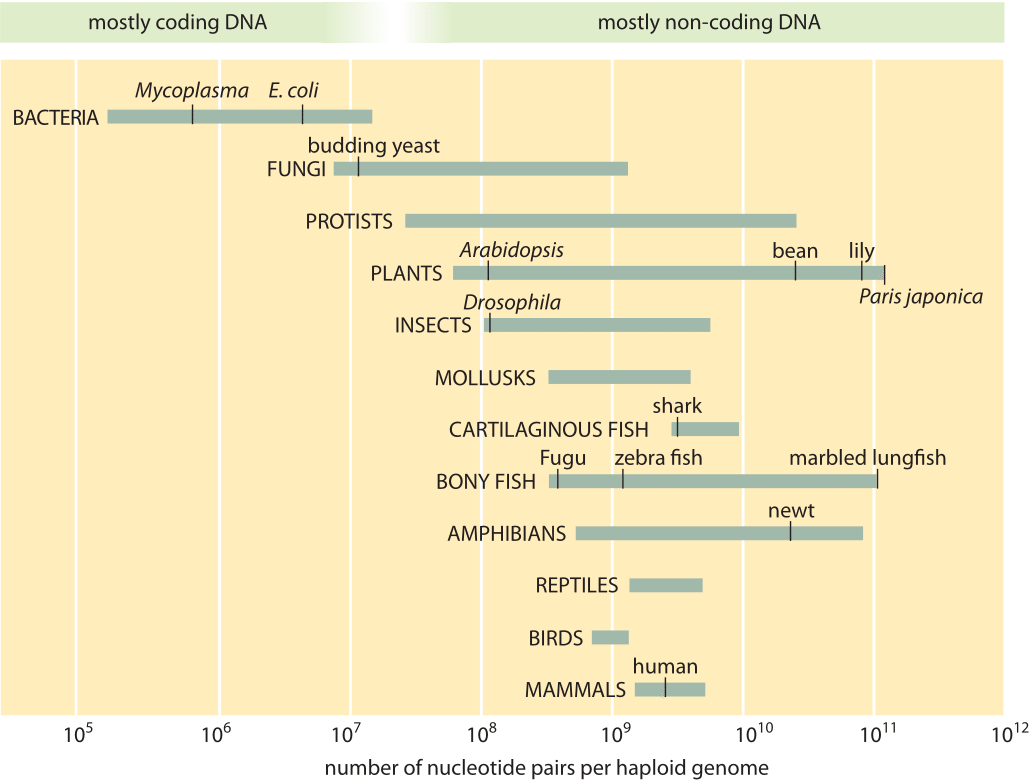
\includegraphics[width=\textwidth]{502-f1-GenomeSizesRanges-1.png}
	\caption{Illustration of the range of genome sizes from \href{http://book.bionumbers.org/size-and-geometry-introduction/}{book.bionumbers.org}}
	\label{fig:genome_sizes}
\end{figure}

It is instructive to compare cell dimensions versus the length of the DNA molecule that needs to fit inside:
\begin{itemize}
  \item $10^{-6}$m (1um): length of a phage genome.
  \item $10^{-3}$m (1mm): length of the bacterial genome ($3\times 10^9$ bases a 0.3nm each)
  \item $1$m (1m): length of the human genome ($3\times 10^9$ bases a 0.3nm each)
\end{itemize}

We see that DNA is much longer than the containing cells, see Fig.~\ref{fig:DNA_packing_illustration}.
An amusing little calculation: if DNA from all $10^{13}$ cells of a human body was strung together, it would cover the distance to the sun ($1.5\times 10^{11}$m) more than 100 fold (accounting for the diploid nature).

\begin{figure}[tb]
	\centering
	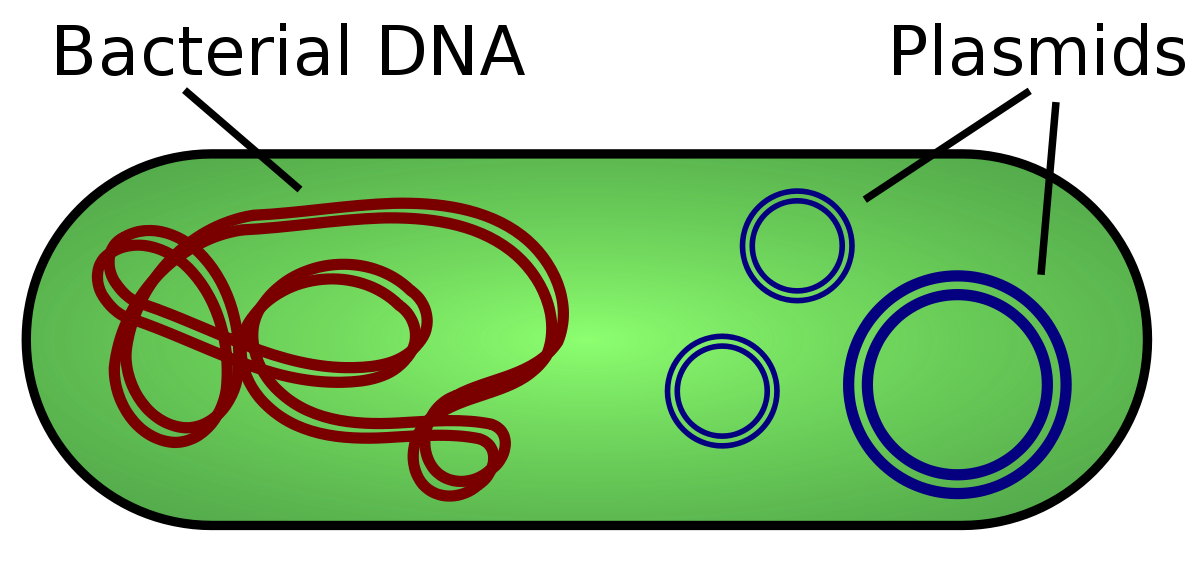
\includegraphics[width=0.6\textwidth]{bacterial_genome}
	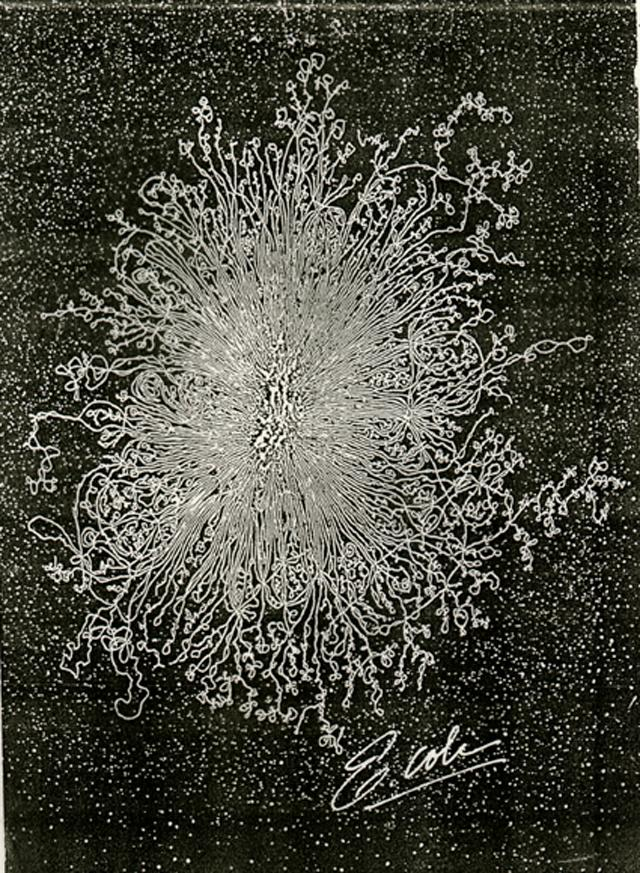
\includegraphics[width=0.25\textwidth]{lysed_ecoli}
	\caption{Left: a typical cartoon suggesting the length of a bacterial chromosome is similar to the length of the cell. Image source: \href{https://www.kissclipart.com/bacterial-genome-clipart-plasmid-genome-bacteria-dt3adi/}{kissclipart}.
	Right: The DNA from an actual E.~coli cell that was lysed (the blob in the middle). A bacterial chromosome of length $5\times 10^6$bps is about 1.5mm long -- roughly 1000-fold the length of the cell.  Clearly, the DNA has to be pretty tightly packed inside the cell. Image source: \href{https://www.nature.com/scitable/content/supercoiled-chromosome-of-e-coli-44517/}{R. Kavanoff}}
	\label{fig:DNA_packing_illustration}
\end{figure}


\subsection{Forces and energies}
So far, we have looked at dimensions and the objects involved could have been dead or alive.
Lets now turn to the energies, power, and forces.
From our daily life, we are used to power on the scale of 100W. This would be your standard (old fashioned) light bulb or the typical power consumption of the human body.
Energy is stored in batteries, reservoirs, or petrol.
In cells, the energy currencies are very different.
The ultimate source of energy (free energy, really) is the sun.
It emits black body radiation at a temperature of 5800K which corresponds to an emission maximum at a wavelength of 550nm in the visible range.
A single photon with wavelength $ \lambda = 500nm$ has the following energy:
\begin{equation}
E = \frac{hc}{\lambda}\approx \frac{1.24 eV\mu m}{\lambda}\approx 2.5eV
\end{equation}
Electron volt (eV) is a unit of energy commonly used in physics. One eV corresponds to the energy required to move one election one Volt up in an electric potential.
Chemists like to measure energy per molecule or reaction and typically use units like $kJ/mol$ or $kcal/mol$.
In a biological system, different energy units are often more convenient.
The most important energy scales in biological systems are the thermal energy kT and the energy released when hydrolyzing ATP to ADP.
The scale kT is important since process that operate on the scale of kT or below happen spontaneously and reversibly, that is they are strongly affected by the randomness to thermal noise.
Controlled and precise reactions typically involve energy differences larger than kT.
Hence it is always important consider an energy difference in relation to kT
\begin{equation}
	kT \approx 0.025eV \approx 0.6 kcal/mol \approx 2.5 kJ/mol \approx 4pN \times nm
\end{equation}
One visible photon is therefore about 100kT, much more than the thermal energy scale.
It is thus plausible that individual visible photons can drive biological processes such as trigger signaling cascades.
To fix one $CO_2$ molecule, around 8 such photons are needed.

The dominant energy currency of the cell is ATP which is hydrolyzed to ADP to power other reactions
\begin{equation}
ATP + H_2O \rightarrow ADP + P_i \quad -30 kJ/mol \approx -12kT
\end{equation}
Again, one ATP hydrolysis is above the thermal energy scale, but not all that far away.
In practice, the (free) energy released in ATP hydrolysis can vary by a factor of two depending on Mg${}^{2+}$ concentration and the concentrations of ATP and ADP.

\begin{figure}[t]
	\centering
	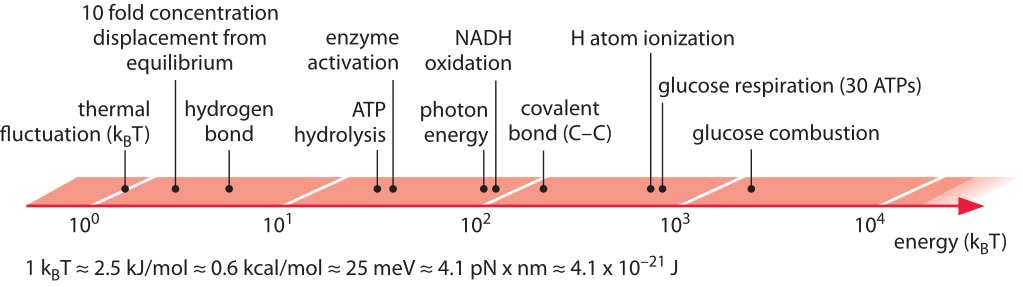
\includegraphics[width=\textwidth]{300-f1-EnergyAxis-11.png}
	\caption{Illustration of the range energy scales from \href{http://book.bionumbers.org/size-and-geometry-introduction/}{book.bionumbers.org}}
	\label{fig:genome_sizes}
\end{figure}


\subsection{Concentrations and molecule counts}
Concentrations are statements about the number of molecules per volume.
There are typically measured as moles per liter, that is $6\times 10^{23}$ molecules per $10^{-3}m^{3}$.
For our purposes, it is useful to express this as number of molecules per femtoliter or $\mu m^3$: 1M=$6\times 10^{23}/10^{15}\mu m^3 = 6\times 10^{8}/\mu m^3$
Hence one nM corresponds to roughly one molecule per bacterium, pM to one molecule per eukaryotic cell.
If proteins are only present in small numbers inside cells or organelles, their individual behavior and the associated stochasticity can be very important.
When thinking about rare molecules, for example signaling molecules, numbers are a better guide than concentrations.

\begin{figure}[h]
	\centering
	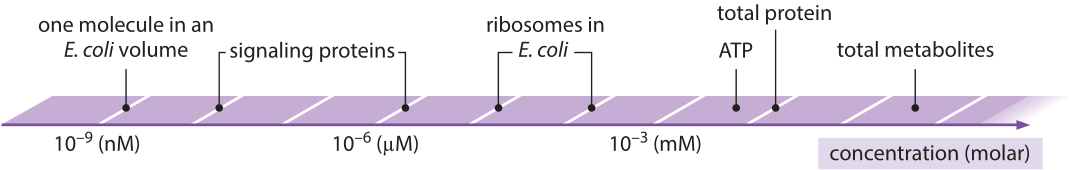
\includegraphics[width=\textwidth]{200-f1-ConcentrationAxis-11.png}
	\caption{Illustration of the range concentrations from \href{http://book.bionumbers.org/size-and-geometry-introduction/}{book.bionumbers.org}}
	\label{fig:genome_sizes}
\end{figure}

% \subsubsection{Stochasticity of molecule numbers}
% Fluctuations are important, when molecules are rare.
% But how much do we expect molecule number to fluctuate?
% Consider a simple process where molecules are added at random times with rate $b$ and decay with rate $d$.
% \begin{equation}
% \begin{split}
% 	n &\rightarrow n+1 \quad \mathrm{with\ rate}\ b \\
% 	n &\rightarrow n-1 \quad \mathrm{with\ rate}\ nd
% \end{split}
% \end{equation}
% There are two things to note here:
% (i) Rates have units of 1/time. In a short time interval $dt$ we expect on average $b\ dt$ new molecules to be produced.
% (ii) The production rate is independent of $n$, while the decay rate increases with $n$ since each particle can decay on its own.
% Intuitively, one expects a balance between production and decay such that the number of molecules settles at a value where these two rates match
% \begin{equation}
% 	b = d \bar{n} \quad \Rightarrow \bar{n} = \frac{b}{d}
% \end{equation}
% This results makes sense: $\bar{n}$ increases with increasing production and decreases with increasing decay rate.
% It happens to be the correct expression for the average number of particles $\bar{n}$.
% When $\bar{n}$ is small, however, the actual number of particles will fluctuate a lot around the average value.
% Such stochasticity is captured by a probability distribution $p(n)$.
% At steady state, we the rates between $n$ and $n+1$ need to balance each other.
% \begin{equation}
% 	p(n-1) b = dn p(n) \quad \Rightarrow \quad p(n) = \frac{b}{dn}p(n-1)
% \end{equation}
% This condition has a simple solution:
% \begin{equation}
% 	p(n) = \frac{(b/d)^n}{n!}e^{-b/d}
% \end{equation}
% This distribution is known as the Poisson distribution, where $n!=n(n-1)(n-2)\ldots 1$ is the factorial.
% It has mean $\bar{n} = b/d$ and variance $\sigma^2 = \bar{n}$ (verification is left as exercise).
% The fact that the variance equals the mean is extremely important.
% The variance is the average squared deviation from the mean.
% The typical deviation from the mean is therefore the square root of the variance.
% This relationship -- noise increasing with the square root of the signal -- is very general and underlies most statistical analysis methods.

\subsubsection{Concentrations, energy, and entropy}
Like temperature, concentrations tend to homogenize spontaneously: connect two reservoirs with different concentrations and over time the two concentrations will tend towards the average concentration through diffusion of molecules.
This homogeneous state is the state of highest entropy.
We will see later in the course that the mathematics describing the dynamics of concentrations is very similar to that of concentrations.

A central (and often unintuitive) aspect of thermodynamics is the interplay of \emph{Energy} and \emph{Entropy}.
Concentration gradients represent a state of low entropy.
Such concentration differences are ubiquitously exploited in biology to drive processes like nuclear transport, ATP synthesis, or neuronal signaling.
This effect is most obvious when considering solutions of positively and negatively charged ions on two sides of a membrane that is only permeable to ions of one charge (for example protons) and not the other charge.
Now assume that initially on each side of the membrane positively and negatively charged ions are present in equal concentrations and thus balance each other.
If the concentration $c_{left}$ is high on one side and low $c_{right}$ on the other side, the type of ion that can cross the membrane will start flowing from left to right.
With this flux, a potential difference builds up that opposes further ion flux until the ion flux stops.
How high is the final potential difference $\Delta V$ where the entropy gain due to mixing is balanced by the potential difference between the reservoirs?

This can be estimated using results from statistical mechanics.
The energy difference of an ion with charge $l$ in the left and right reservoir will be $l\Delta V$.
The probabilities of observing it on the left or right in equilibrium (assuming everything else is equal) are therefore related by $p_{left}/p_{right} = e^{-l\Delta V/kT}$.
This ratio, however, is exactly the ratio of the equilibrium probabilities (not that the flux of ions is typically so small compared to the overall concentrations that we can treat the latter as constant).
\begin{equation}
	\frac{c_{left}}{c_{right}} = \frac{p_{left}}{p_{right}} = e^{-\frac{l\Delta V}{kT}} \quad \Rightarrow \quad kT \log(c_{left}/c_{right})  = - l\Delta V
\end{equation}
We see that the potential difference is proportional to the logarithm of the concentration difference!
This is the famous Nernst potential.
It directly connects the thermal energy scale $kT$, the entropy (logarithmic concentrations), and the potential energy.

A pH difference of 1 (ten fold difference in $H^+$ ion concentration) then corresponds to a potential difference of
$\log(10) \approx 2.3 kT \approx 0.06 eV$ or $60meV$.
Typical potential differences across membranes are of the order of $100meV$.

\section{Estimating orders of magnitude}

\subsection{Molecular motors}
Cells have molecular motors that they use to move things around, drive cilia and flagella, or open up the DNA double strand.
Most of these hydrolyze ATP, one molecule at a time.
Some of these motors (kinesin and dynein) move in steps along filaments.
These steps are on the order of 10nm.
Assuming the energy of one ATP hydrolysis is converted with 100\% efficiency into mechanical energy, we expect a maximum force (stall force) of

\begin{equation}
\frac{12kT}{10nm} \approx \frac{48pN nM}{10nm} \approx 5pN
\end{equation}

This estimate is surprisingly accurate -- most ``walking'' molecular motors have \href{http://bionumbers.hms.harvard.edu/bionumber.aspx?&id=112209&ver=1&trm=stall%20force}{stall forces in this range}.


\subsection{Genome replication}
If a genome has a single origin of replication, the rate of genome replication $\kappa$, genome size $L$, and division time $\tau$ are naively related by

\begin{equation}
\kappa = \frac{L}{\tau} = \frac{5\times 10^{6}}{2500s} \approx 2\times 10^3/s
\end{equation}
where we have used a typical bacterial genome size of 5Mb and a division time of 40min.
2000 bases per second is not far off, but probably a factor of 5 too high.
Furthermore, E.~coli can divide in 20min rather than 40min.
The discrepancy can resolved by observing that (i) replication proceeds via two replication forks, and (ii) the next replication is started before the first one is complete.

Eukaryotic replication machinery is no faster than the prokaryotic ones, but the genomes are 1000 fold larger.
To replicate their genomes in reasonable time eukaryotic genomes have 1000s of origins of replication.

\subsection{Take home messages}

\begin{itemize}
    \item For quantitative reasoning, it is important to have a sense of the relevant scales!
    \item Simple ``back-of-the-envelope" calculation can give you important insights into the nature of a problem
    \item Many processes in biology happen at low copy numbers and with energies close to $kT$. Stochastic effects are important.
\end{itemize}

\section{Differential equations}
Mathematics, and differential equations in particular, are the language suitable to describe, analyze, and predict quantitative phenomena.
Some knowledge of differential equations is essential, and this should have been covered in high school and last year's courses.

There are many excellent treatise of differential equations out there.
We will review this topic and discuss how such equations are solved numerically in the lecture.



% \subsection{The number of ribosomes}
% In an exponentially growing bacterial culture, biomass doubles once every division time.
% About one fourth of the cell mass is protein, which comes down to
% \begin{equation}
% N_{aa} = 0.25 \times 10^{-12} g/cell \times 6\times 10^{23} \frac{Da}{g} / 100 \frac{aa}{Da} \approx 10^9 aa/cell
% \end{equation}
% amino acids per cell that need to be synthesized every 20min and incorporated in to peptides.
% Peptide synthesis rate of 10aa/s, a single ribosome can process about $10^4$ amino acids per cell cycle, suggesting the cell needs at about $10^5$ ribosomes.
% This is roughly what is measured. Again, \href{http://book.bionumbers.org/how-many-ribosomes-are-in-a-cell/}{bionumbers.org} has a very nice description of this problem.
% Importantly, this quick calculation tells us that ribosomes make up a substantial fraction of the total cell proteome (they certainly dominate the RNA pool).

